% arara: xelatex: { synctex: yes, shell: yes }
\documentclass[palatino]{ist-report}

\usepackage{amssymb}
\usepackage{gensymb}
\usepackage{booktabs}
\usepackage{placeins}

% -- Bibliografia
\usepackage[
	backend = biber,
	style = numeric,
	sorting = ynt
	]{biblatex}
\addbibresource{main.bib}
\usepackage{fvextra}
\usepackage{csquotes}

\usepackage{minted}
\definecolor{bg}{rgb}{0.95,0.95,0.95}
\setminted{linenos, bgcolor = bg, breaklines}
\setmintedinline{bgcolor = {}}

\graphicspath{{graphics/}}

\settitle{Projeto Final}
\setsubtitle{GPS -- Mínimos Quadrados e EKF Modelo PV}
\setcourse{Sistemas de Controlo de Tráfego}
\setsubject{Mestrado Integrado em Engenharia Aeroespacial}
\author{Pedro Afonso \\ \texttt{66277} \and João Manito \\ \texttt{73096}}

\begin{document}

\makecover

\begin{abstract}
    O projeto aqui descrito consistiu na estimação da trajetória de uma aeronave por GPS e o seu comportamento na variação de satélites presentes e considerações de imperfeições na atmosfera. Para auxiliar na optimização do trabalho implementaram-se algoritmos de mínimos quadrados e \textit{Extended Kalman Filter} para a minimização de ruído atmosférico  e estimação de vários parâmetros da trajetória da aeronave com base nos dados obtidos por GPS.
\end{abstract}

{\hypersetup{linkcolor = {black}}\tableofcontents}

\pagebreak

\section{Introdução}

O objectivo deste trabalho teve como aplicação dois métodos diferentes utilizados por um receptor GPS, o \textit{Extended Kalman Filter} com o modelo Posição e Velocidade bem como o Método dos mínimos quadrados. 

A avaliação destes dois métodos exige uma simulação e posterior comparação entre os valores estimados e valores reais. 
Para a simulação foi necessário cálculo orbital, para obtenção da posição de cada satélite em cada instante de tempo, utilizando um ficheiro de almanaque em formato \textit{Yuma}.

É possível calcular também a velocidade instantânea do GPS em cada instante, revelando-se uma grande utilidade.

A base de cálculo da posição do receptor baseia-se no tempo que demora a viajar um sinal emitido por um satélite de forma a que multiplicado pela constante da velocidade da luz, indique a distância (com erros de vários tipos) a que se encontra o receptor daquele satélite. Através da triangulação é possível estimar a posição do receptor. Note-se que para aplicar a triangulação são precisos pelo menos 4 satélites.

\pagebreak

\section{Constelação}
De forma a conseguir realizar o presente projecto, foi necessário obter um conjunto de pseudo-distâncias  entre os satélites da constelação de GPS e o receptor. Para tal, foi criada uma rotina que simula o o movimento destes satélites, permitindo obter a sua distância ao receptor e eventual cálculo das pseudo-distâncias.

De forma a conseguir obter os parâmetros orbitais necessários à simulação da constelação, usaram-se os dados do almanaque de GPS em formato \textit{Yuma}, obtidos através do \textit{website Celestrak}. 

Para a constelação de GPS, os parâmetros orbitais podem ser encontrados na tabela \ref{tab:parametros_orbitais_GPS}.

\begin{table}[ht]
    \centering
    \begin{tabular}{c c}\toprule
        \textbf{Parâmetro} & \textbf{Valor} \\
        \midrule
        $\mu$ & $3.986005\times10^{14}\,m^3s^{-1}$ \\
        $A$ & $2.65617\times10^{7}\,m$\\
        $e_0$ & $0$\\
        $T$ & $43082\,s$ \\
        $R$ & $26559800\,m$ \\
        $\alpha$ & $55\,\degree$ \\
        \bottomrule
    \end{tabular}
    \caption{Parâmetros orbitais da constelação de GPS}
    \label{tab:parametros_orbitais_GPS}
\end{table}

Estes parâmetros não são os parâmetros reais da constelação, mas são uma boa aproximação dos mesmos. Usando esta aproximação, podemos então calcular as coordenadas de cada satélite. Definindo $\Delta t = t_{st} - t_{oe}$, em que $t_{st}$ é o tempo de transmissão e $t_{oe}$ o tempo de referência da efeméride (neste caso igual ao tempo de aplicabilidade do almanaque) obtemos
\begin{equation*}
    \theta = \theta_0 + \frac{360}{T}\Delta t
\end{equation*}

\begin{equation*}
    \Omega = \Omega_0 + \frac{360}{2T}t_{st}
\end{equation*}

No presente projecto foi considerado que o tempo de transmissão é aproximadamente igual ao tempo de simulação. Como a velocidade de propagação da luz no vácuo é bastante elevada relativamente à velocidade orbital do satélite o erro derivado desta aproximação é baixo.

Para calcular a distância do receptor aos satélites é necessário saber a posição de cada satélite num referencial ECEF. A posição aproximada de um satélite no referencial ECEF é dada por:
\begin{gather*}
    \left[\begin{matrix}
        x \\ y \\ z
    \end{matrix}\right]
    = R
    \left[\begin{matrix}
        \cos\theta\cos\Omega - \sin\theta\sin\Omega\cos\alpha \\
        \cos\theta\sin\Omega + \sin\theta\cos\Omega\cos\alpha \\
        \sin\theta\sin\alpha
    \end{matrix}\right]
\end{gather*}

Podemos então calcular a distância real entre satélite e receptor pela fórmula
\begin{gather}\label{eq:rhon}
    R = \sqrt{(X_N - x_u)^2 + (Y_N-y_u)^2 + (Z_N - z_u)^2}
\end{gather}

Por fim podemos obter a pseudo-distância 
\begin{gather}\label{eq:rhon}
    \rho_N = R + \rho_{iono,n} + n_m(t)
\end{gather}

em que $\rho_{iono,n}$ é o erro devido às perturbações ionosféricas e $n_m(t)$ é ruído aditivo gaussiano branco, de média nula e variância $\sigma^2_{noise}$.

\begin{figure}[ht]
	\centering
	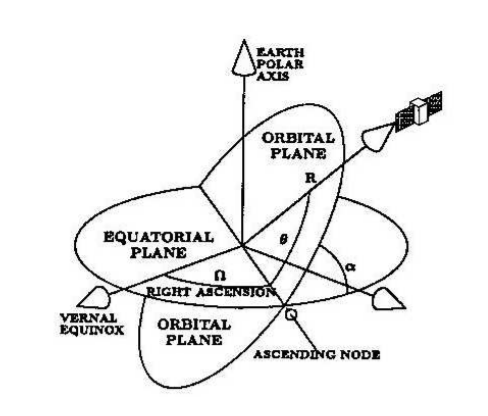
\includegraphics[width=0.6\textwidth]{graphics/satelites.png}
	\caption{Coordenadas dos satélites}
	\label{satelite}
\end{figure}

%\begin{gather}\label{eq:rhon}
%    \rho_N = \sqrt{(X_N - x_u)^2 + (Y_N-y_u)^2 + (Z_N - z_u)^2} + c t_u + \epsilon
%\end{gather}








\pagebreak

\section{Método dos Mínimos Quadrados}

Utilizando a equação \ref{eq:rhon}, desprezámos os valores do erro $\epsilon$ e simplificámos a expressão $ct_u$ com o termo $b_u = ct_u$. Desenvolvemos assim o modelo incremental da equação \ref{eq:inc}.
\begin{gather}\label{eq:inc}
    \Delta \rho_i = \frac{\partial\rho_i}{\rho x_u}\Delta x_u + \frac{\partial\rho_i}{\rho y_u}\Delta y_u + \frac{\partial\rho_i}{\rho z_u}\Delta z_u
\end{gather}
A forma matricial é visível na equação \ref{eq:matr}, cujas matrizes podem ser vistas na equação \ref{eq:matr_each}.
\begin{subequations}
\begin{gather}
    \Delta\rho = G\Delta X \label{eq:matr} \\
    \Delta\rho = \left[\begin{matrix}\Delta\rho_1 \\ \vdots \\ \Delta\rho_N\end{matrix}\right], \quad \Delta X = \left[\begin{matrix}\Delta x_u \\ \Delta y_u \\ \Delta z_u \\ \Delta b_u\end{matrix}\right], \quad G = \left[\begin{matrix}
        \frac{\partial\rho_1}{\partial x_u} & \frac{\partial\rho_1}{\partial y_u} & \frac{\partial\rho_1}{\partial z_u} & 1 \\
        \vdots & \vdots & \vdots & \vdots \\
        \frac{\partial\rho_N}{\partial x_u} & \frac{\partial\rho_N}{\partial y_u} & \frac{\partial\rho_N}{\partial z_u} & 1 \\
    \end{matrix}\right] \label{eq:matr_each}
\end{gather}
\end{subequations}
Cada derivada parcial da matriz $G$ da equação \ref{eq:matr_each} pode ser descrita como visível nas equações em \ref{eq:partial}.
\begin{subequations}
\begin{gather}\label{eq:partial}
    \frac{\partial\rho_i}{\partial x_u} = -\frac{X_i - x_u}{D_i}, \quad \frac{\partial\rho_i}{\partial y_u} = -\frac{Y_i - x_u}{D_i}, \quad \frac{\partial\rho_i}{\partial z_u} = -\frac{Z_i - x_u}{D_i} \\
    D_i = \sqrt{(X_i - x_u)^2 + (Y_i - y_u)^2 + (Z_i - z_u)^2}
\end{gather}
\end{subequations}
O vetor $\Delta X$ pode ser determinado via o \textbf{método dos mínimos quadrados}, que para o problema em questão se encontra descrito na equação \ref{eq:ls}.
\begin{gather*}\label{eq:ls}
    \Delta X = \left(G^TG\right)^{-1}G^T\Delta\rho
\end{gather*}


\begin{figure}[ht]
	\centering
	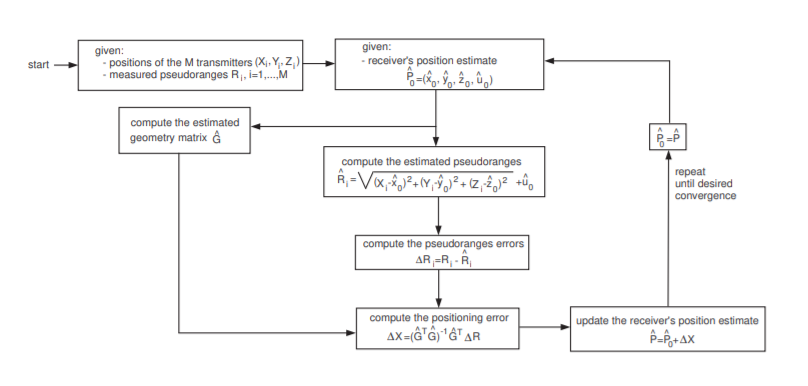
\includegraphics[width=0.8\textwidth]{graphics/minimosquadrados.png}
	\caption{Algoritmos do método dos mínimos quadrados}
	\label{LS}
\end{figure}




\section{\textit{Extended Kalman Filter} -- Modelo PV}

O Fluxograma do filtro de Kalman generalizado, aplicado à resolução da equação de navegação em GPS em que o intervalo de tempo das iterações foi de $ \delta t = 1 s$ está representado na figura abaixo, \ref{kalman}.


\begin{figure}[ht]
	\centering
	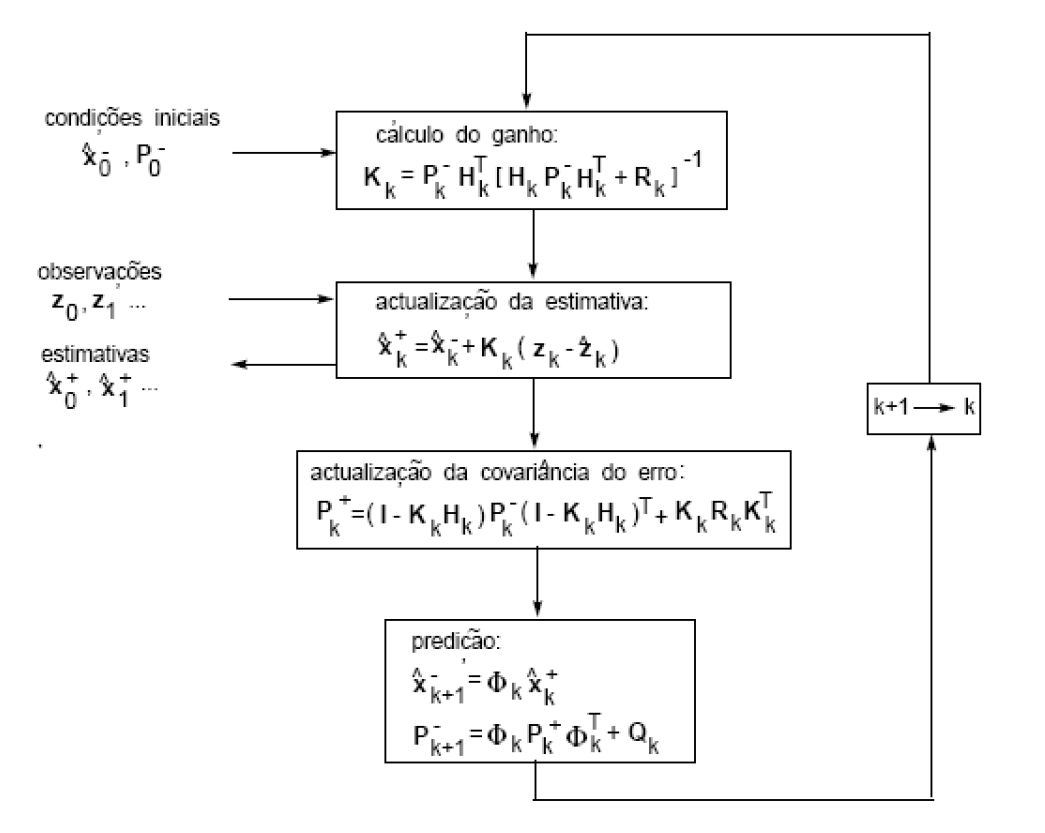
\includegraphics[width=0.6\textwidth]{graphics/kalman.png}
	\caption{Algoritmo do \textit{Extended Kalman filter}.}
	\label{kalman}
\end{figure}

Em que $x_0^-$ é a estimativa inicial das condições da dinâmica, e $P_0^-$ é a matriz da covariância da filtragem inicial. $K_k$ é o ganho de Kalman e é calculado tal como se exemplifica na figura. $z_0,z_1,..z_n$ são as pseudo-distâncias medidas e $x_0^+,x_1^+$ as estimativas da posição ao longo das iterações. O modelo seguido é com os estados de posição, velocidade e os dois estados extra relativos ao relógio. O erro do relógio do receptor pode induzir erros significativos no cálculo da posição. 

O relógio do receptor consiste num oscilador de quartzo convencional e admite-se que este se encontra sincronizado no início da simulação, sendo por isso o modelo de estado do relógio o da figura \ref{relogio}, em que $\delta T$ é o desvio entre o tempo de relógio do receptor e do sistema GPS.


\begin{figure}[ht]
	\centering
	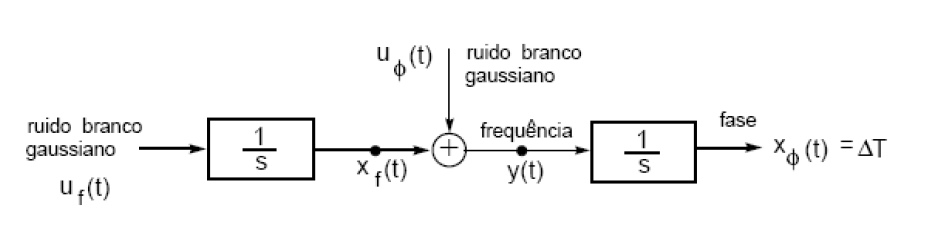
\includegraphics[width=0.8\textwidth]{graphics/relogio.png}
	\caption{Modelo de estado do relógio do receptor.}
	\label{relogio}
\end{figure}


O nosso modelo em tempo discreto, em espaço de estados fica:

\begin{align}
\begin{bmatrix} x_{1,k+1} \\ x_{2,k+1} \\ x_{3,k+1} \\ x_{4,k+1}\\ x_{5,k+1}\\ x_{6,k+1} \\ x_{7,k+1} \\ x_{8,k+1} \end{bmatrix}
= \begin{bmatrix}
1 & \Delta t & 0 & 0 & 0 & 0 & 0 & 0 \\
0 & 1 & 0 & 0 & 0 & 0 & 0 & 0 \\
0 & 0 & 1 & \Delta t & 0 & 0 & 0 & 0 \\
0 & 0 & 0 & 1 & 0 & 0 & 0 & 0 \\
0 & 0 & 0 & 0 & 1 & \Delta t & 0 & 0 \\
0 & 0 & 0 & 0 & 0 & 1 & 0 & 0 \\
0 & 0 & 0 & 0 & 0 & 0 & 1 & \Delta t \\
0 & 0 & 0 & 0 & 0 & 0 & 0 & 1
\end{bmatrix} 
\begin{bmatrix} x_{1,k} \\ x_{2,k} \\ x_{3,k} \\ x_{4,k}\\ x_{5,k}\\ x_{6,k} \\ x_{7,k} \\ x_{8,k} \end{bmatrix} + \begin{bmatrix} u_{1,k} \\ u_{2,k} \\ u_{3,k} \\ u_{4,k}\\ u_{5,k}\\ u_{6,k} \\ u_{7,k} \\ u_{8,k} \end{bmatrix}
\end{align}

Por sua vez, a matriz covariância do ruído dá:
%\vspace*{2cm}
\begin{align}
Q
= \begin{bmatrix}
q_v \frac{(\Delta t)^3}{3} & q_v \frac{(\Delta t)^2}{2}  & 0 & 0 & 0 & 0 & 0 & 0 \\
\frac{(\Delta t)^2}{2} & q_v (\Delta t) & 0 & 0 & 0 & 0 & 0 & 0 \\
0 & 0 & q_v \frac{(\Delta t)^3}{3} & q_v \frac{(\Delta t)^2}{2} & 0 & 0 & 0 & 0 \\
0 & 0 & q_v \frac{(\Delta t)^2}{2} & q_v (\Delta t)  & 0 & 0 & 0 & 0 \\
0 & 0 & 0 & 0 & q_v\frac{(\Delta t)^3}{3} & q_v\frac{(\Delta t)^2}{2} & 0 & 0 \\
0 & 0 & 0 & 0 & q_v\frac{(\Delta t)^2}{2} & q_v (\Delta t) & 0 & 0 \\
0 & 0 & 0 & 0 & 0 & 0 & (q_{\phi}\Delta t + q_f \frac{(\Delta t)^3 }{3})c^2 & q_f \frac{(\Delta t)^2}{2} c^2 \\
0 & 0 & 0 & 0 & 0 & 0 & q_f \frac{(\Delta t)^2}{2}c^2 & q_f c^2 (\Delta t)
\end{bmatrix} 
\end{align}
Em que $\Delta t$ é o inverso da frequência de amostragem, portanto $1$ segundo e $q_v$ consideramos com o valor $10$. Os restantes valores da matriz são dados por:

\begin{equation*}
    q_{\phi} = \frac{h_0}{2} = 10^{-19}
\end{equation*}
  
\begin{equation*}
      q_f = 3.95 \times 10^{-19}
\end{equation*}

\subsection{Modelo de observações}

O valor de $z_k=[\rho_{1,k},...,\rho_{n,k}]$ representa o vector das pseudo distâncias medidas e fornecidas como input ao EKF. 


\begin{equation*}
    z_k = h(x(t_k))+v_k
\end{equation*}


Agora podemos definir a matriz h, em que 


\begin{gather*}
    h(x) = \left[\begin{matrix}
        \sqrt{(\Tilde{x_1} - x_a)^2 + (\Tilde{y_1}-y_u)^2 + (\Tilde{z_1} - x_c)^2} + x_d \\
        \vdots \\
       \sqrt{(\Tilde{x_N} - x_a)^2 + (\Tilde{y_N}-x_b)^2 + (\Tilde{z_N} - x_c)^2} + x_d
    \end{matrix}\right]
\end{gather*}


A matriz R, conhecida por matriz de covariância do ruído das observações é dada por uma matriz diagonal $(n x n)$ (em que n é o número de satélites que estão a enviar informação acerca dos pseudoranges), $R_k=\sigma_{UERE}^2 I$:


\begin{align*}
\begin{bmatrix}
\sigma_{UERE}^2 & 0 & 0 & \hdots \\
0 & \sigma_{UERE}^2 & 0 & \hdots \\
0 & 0 & \sigma_{UERE}^2 & \hdots \\
\vdots & \vdots & \vdots & \ddots
\end{bmatrix} 
\end{align*}

A matriz H usada pelo extended Kalman Filter é dada por:


\begin{equation*}
    H_k = \left[\frac{\partial h_i [\hat{x}(k|k-1)]}{\partial x_j}\right]
\end{equation*}

A sua determinação para cada iteração encontra-se escrita no código. 


\subsection{Simulações}

De seguida apresentamos os resultados para as simulações efecutadas. Nas Figuras \ref{real1} e \ref{real2} podemos ver a trajectória efectuada pela aeronave, tanto em coordenadas cartesianas no plano N-E como em latitude e longitude.

\begin{figure}[ht]
	\centering
	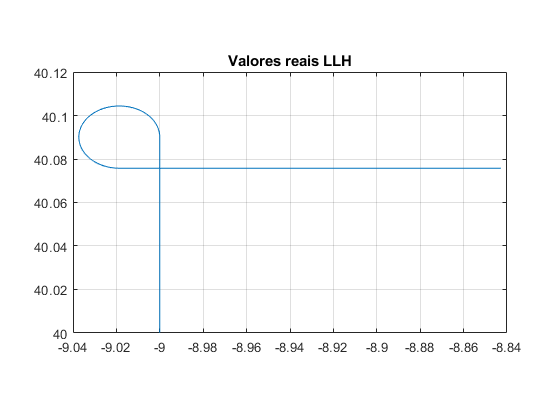
\includegraphics[width=0.7\textwidth,trim={0 15mm 0 12mm},clip]{graphics/plot_posicao_real_LLH11.png}
	\caption{Trajectória real da aeronave para comparação com as trajectórias estimadas.}
	\label{real1}
\end{figure}

\begin{figure}[ht]
	\centering
	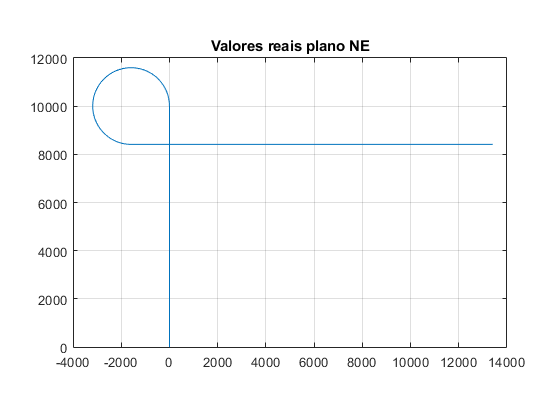
\includegraphics[width=0.7\textwidth,trim={0 18mm 0 0},clip]{graphics/realnascondicoesdoproblema.png}
	\caption{Posições da trajectória real nas condições do problema, coordenadas Norte Este.}
	\label{real2}
\end{figure}

\begin{figure}[ht]
	\centering
	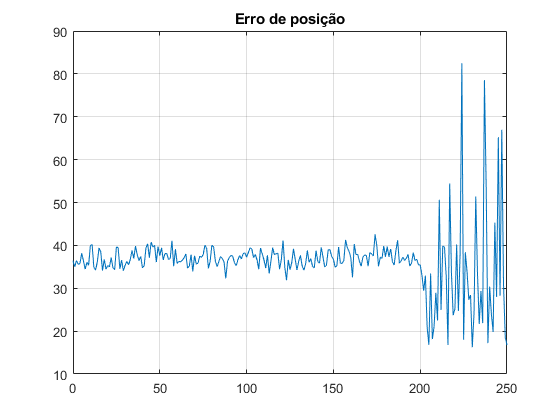
\includegraphics[width=0.7\textwidth,trim={0 7mm 0 0},clip]{graphics/erro_posicao11.png}
	\caption{Erro de posição do método dos mínimos quadrados com Ionosfera e com Canyon.}
	\label{pos11}
\end{figure}


\begin{figure}[ht]
	\centering
	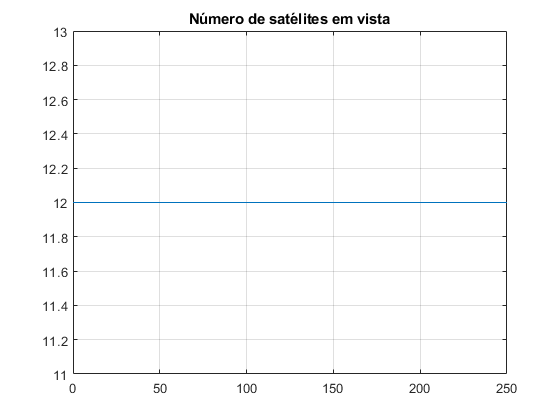
\includegraphics[width=0.7\textwidth,trim={0 7mm 0 0},clip]{graphics/n_sats.png}
	\caption{Número de Satélites em vista.}
	\label{satelites1}
\end{figure}



\begin{figure}[ht]
	\centering
	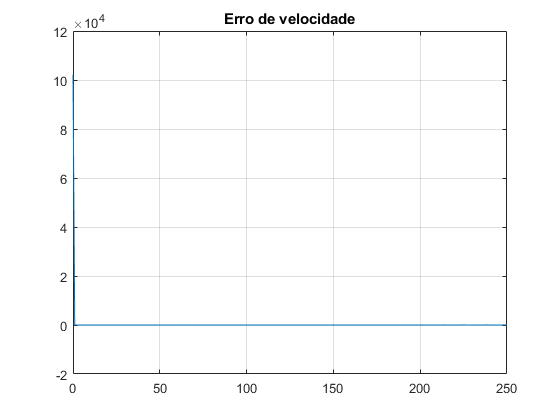
\includegraphics[width=0.7\textwidth,trim={0 5mm 0 0}, clip]{graphics/erro_velocidade11.png}
	\caption{Erro de velocidade do método dos mínimos quadrados com Ionosfera e com Canyon.}
	\label{vls11}
\end{figure}

\begin{figure}[ht]
	\centering
	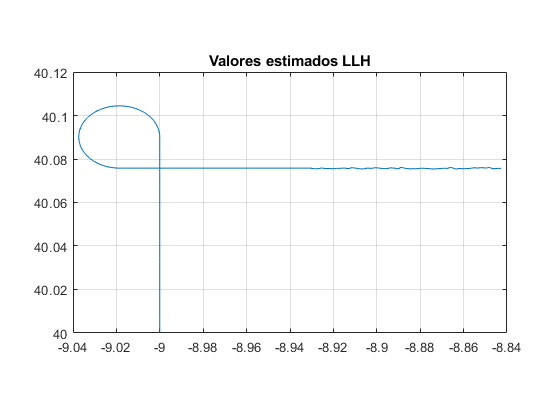
\includegraphics[width = 0.7\textwidth, trim = {7mm 17mm 10mm 10mm}, clip]{graphics/plot_posicao_estimada_LLH11.png}
	\caption{Erro de posição estimada com método dos mínimos quadrados com Ionosfera e com Canyon em latidude e longitude.}
	\label{LLH11}
\end{figure}



\begin{figure}[ht]
	\centering
	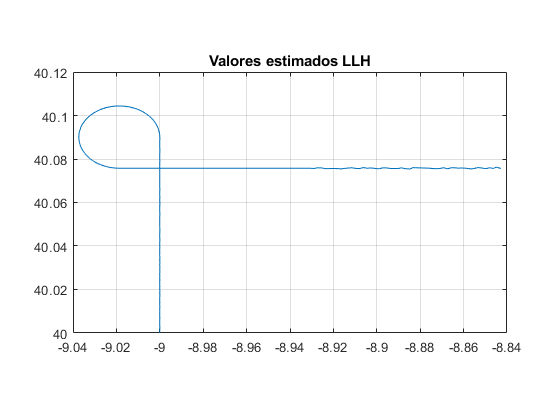
\includegraphics[width=0.6\textwidth]{graphics/plot_posicao_estimada_LLH12.png}
	\caption{Posição estimada com método dos mínimos quadrados sem Ionosfera e com Canyon.}
	\label{posicao12}
\end{figure}



\begin{figure}[ht]
	\centering
	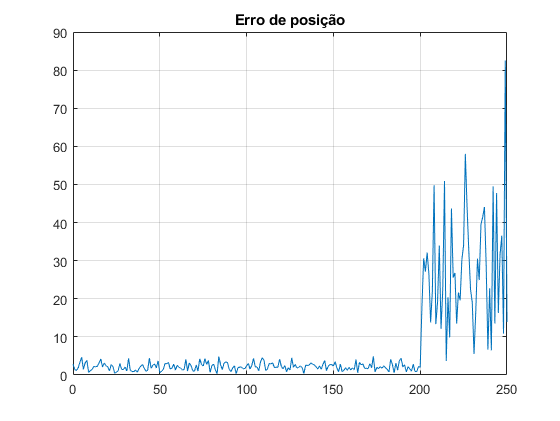
\includegraphics[width=0.6\textwidth]{graphics/erro_posicao12.png}
	\caption{Erro de posição do método dos mínimos quadrados sem Ionosfera e com Canyon.}
	\label{eposicao12}
\end{figure}



\begin{figure}[ht]
	\centering
	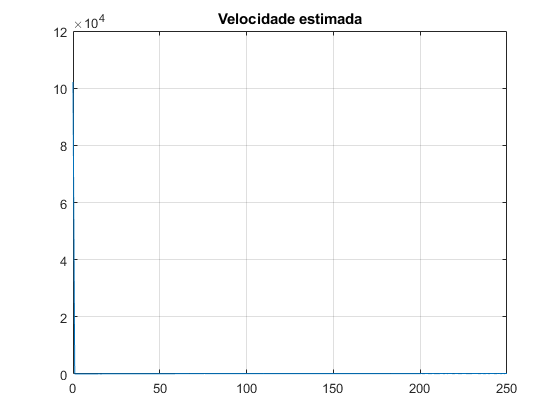
\includegraphics[width=0.6\textwidth]{graphics/velocidade_estimada12.png}
	\caption{Velocidade estimada pelo método dos mínimos quadrados sem Ionosfera e com Canyon.}
	\label{velocidade12}
\end{figure}

\begin{figure}[ht]
	\centering
	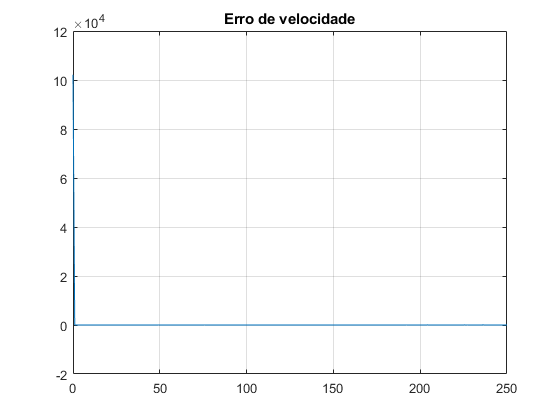
\includegraphics[width=0.6\textwidth]{graphics/errodevelocidade12.png}
	\caption{Erro de velocidade estimada pelo método dos mínimos quadrados sem Ionosfera e com Canyon.}
	\label{evelocidade12}
\end{figure}


\begin{figure}[ht]
	\centering
	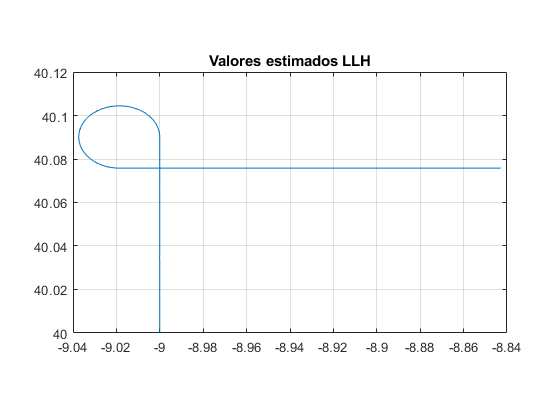
\includegraphics[width=0.6\textwidth]{graphics/plot_posicao_estimada_LLH13.png}
	\caption{Posição estimada pelo método dos mínimos quadrados com Ionosfera e sem Canyon}
	\label{posicao13}
\end{figure}


\begin{figure}[ht]
	\centering
	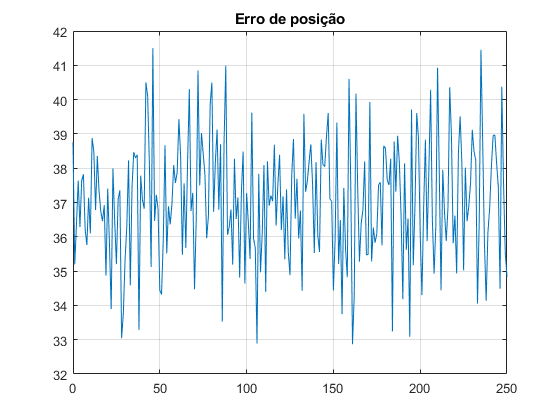
\includegraphics[width=0.6\textwidth]{graphics/erro_posicao13.png}
	\caption{Erro de posição estimada pelo método dos mínimos quadrados com Ionosfera e sem Canyon}
	\label{eposicao13}
\end{figure}


\begin{figure}[ht]
	\centering
	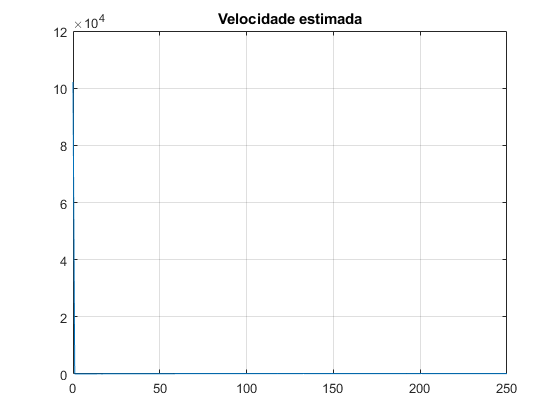
\includegraphics[width=0.6\textwidth]{graphics/velocidade_estimada13.png}
	\caption{Velocidade estimada pelo método dos mínimos quadrados com Ionosfera e sem Canyon}
	\label{Velocidade13}
\end{figure}


\begin{figure}[ht]
	\centering
	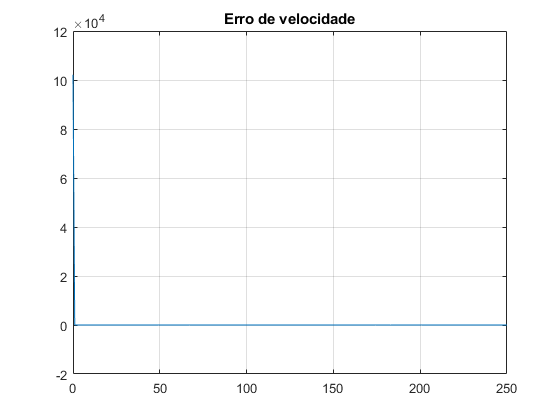
\includegraphics[width=0.6\textwidth]{graphics/erro_velocidade13.png}
	\caption{Erro de velocidade estimada pelo método dos mínimos quadrados com Ionosfera e sem Canyon}
	\label{eVelocidade13}
\end{figure}


\begin{figure}[ht]
	\centering
	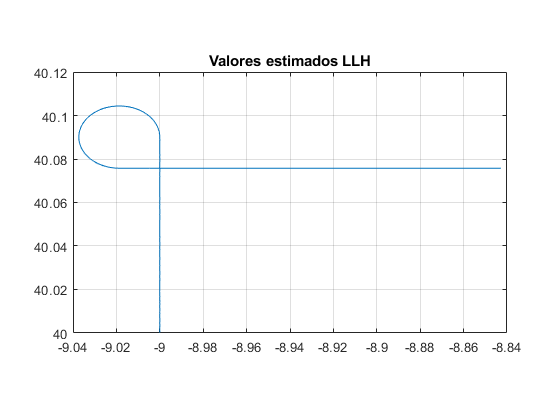
\includegraphics[width=0.6\textwidth]{graphics/plot_posicao_estimada_LLH14.png}
	\caption{Posição estimada pelo método dos mínimos quadrados sem Ionosfera e sem Canyon}
	\label{posicao14}
\end{figure}


\begin{figure}[ht]
	\centering
	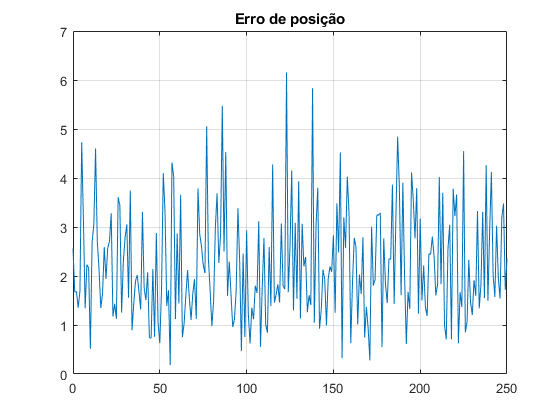
\includegraphics[width=0.6\textwidth]{graphics/erro_posicao14.png}
	\caption{Erro de posição estimada pelo método dos mínimos quadrados sem Ionosfera e sem Canyon}
	\label{eposicao14}
\end{figure}


\begin{figure}[ht]
	\centering
	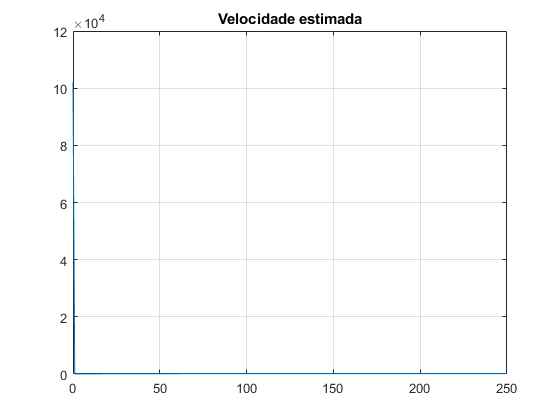
\includegraphics[width=0.6\textwidth]{graphics/velocidade_estimada14.png}
	\caption{Velocidade estimada pelo método dos mínimos quadrados sem Ionosfera e sem Canyon}
	\label{Velocidade14}
\end{figure}


\begin{figure}[ht]
	\centering
	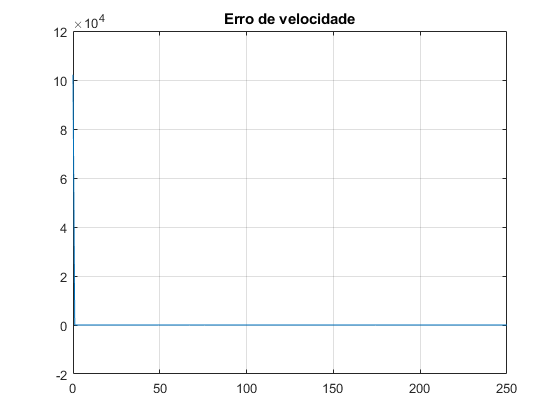
\includegraphics[width=0.6\textwidth]{graphics/erro_velocidade14.png}
	\caption{Erro de Velocidade estimada pelo método dos mínimos quadrados sem Ionosfera e sem Canyon}
	\label{eVelocidade14}
\end{figure}

\begin{figure}[ht]
	\centering
	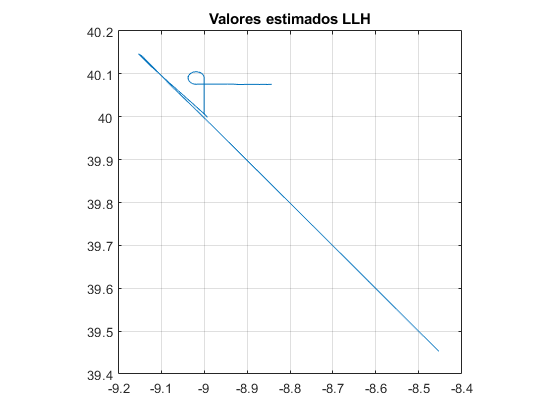
\includegraphics[width=0.8\textwidth]{kalman_1/2-1-plot_posicao_estimada_LLH.png}
	\caption{Kalman, Posição Estimada com Ionosfera e com Canyon.}
	\label{Posicao21}
\end{figure}


\begin{figure}[ht]
	\centering
	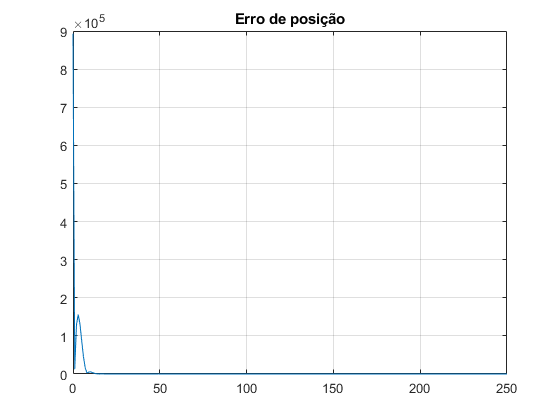
\includegraphics[width=0.8\textwidth]{kalman_1/2-1-erro_posicao.png}
	\caption{Kalman, Erro de Posição Estimada com Ionosfera e com Canyon.}
	\label{EPosicao21}
\end{figure}

\begin{figure}[ht]
	\centering
	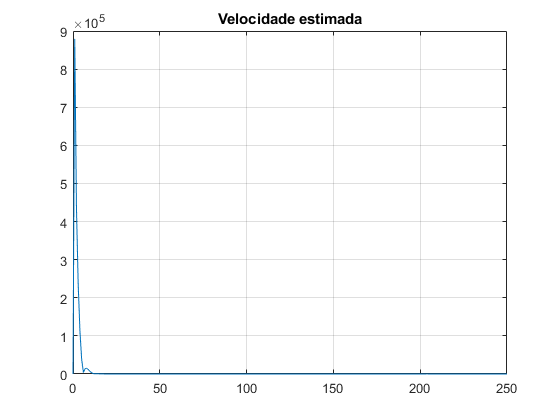
\includegraphics[width=0.8\textwidth]{kalman_1/2-1-velocidade_estimada.png}
	\caption{Kalman, Velocidade Estimada com Ionosfera e com Canyon.}
	\label{Velocidade21}
\end{figure}

\begin{figure}[ht]
	\centering
	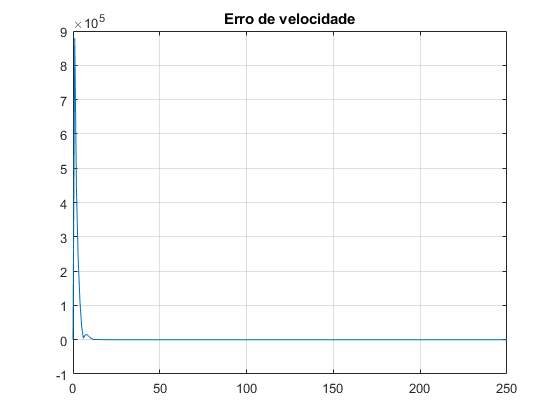
\includegraphics[width=0.8\textwidth]{kalman_1/2-1-erro_velocidade.png}
	\caption{Kalman, Erro de Velocidade Estimada com Ionosfera e com Canyon.}
	\label{eVelocidade21}
\end{figure}


\begin{figure}[ht]
	\centering
	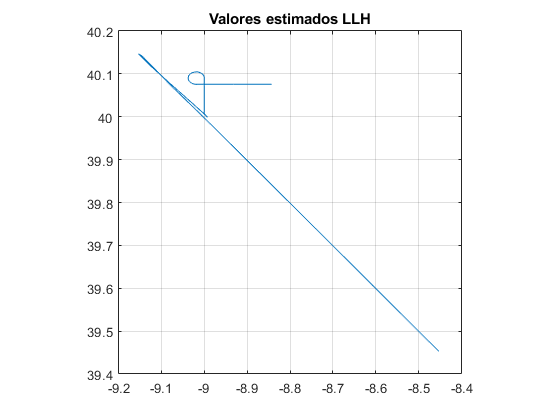
\includegraphics[width=0.8\textwidth]{kalman_2/2-2-plot_posicao_estimada_LLH.png}
	\caption{Kalman, Posição Estimada sem Ionosfera e com Canyon.}
	\label{Posicao22}
\end{figure}

\begin{figure}[ht]
	\centering
	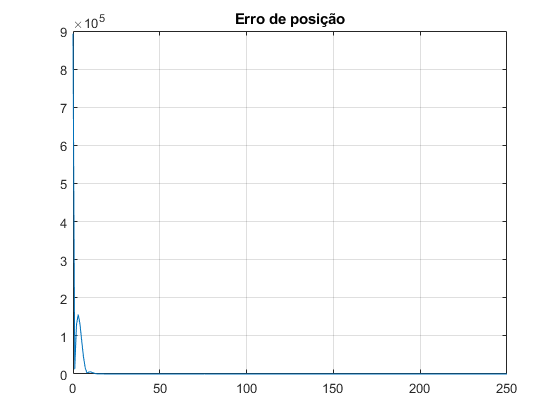
\includegraphics[width=0.8\textwidth]{kalman_2/2-2-erro_posicao.png}
	\caption{Kalman, Erro Posição Estimada sem Ionosfera e com Canyon.}
	\label{ePosicao22}
\end{figure}


\begin{figure}[ht]
	\centering
	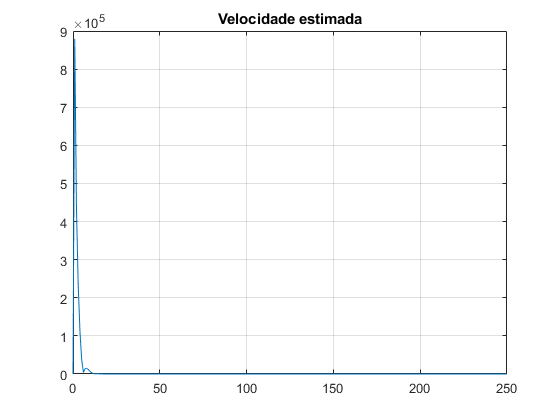
\includegraphics[width=0.8\textwidth]{kalman_2/2-2-velocidade_estimada.png}
	\caption{Kalman, Velocidade Estimada sem Ionosfera e com Canyon.}
	\label{velocidade22}
\end{figure}

\begin{figure}[ht]
	\centering
	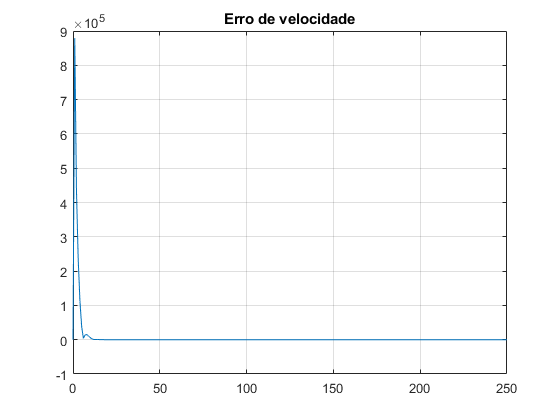
\includegraphics[width=0.8\textwidth]{kalman_2/2-2-erro_velocidade.png}
	\caption{Kalman,Erro de Velocidade Estimada sem Ionosfera e com Canyon.}
	\label{evelocidade22}
\end{figure}

\begin{figure}[ht]
	\centering
	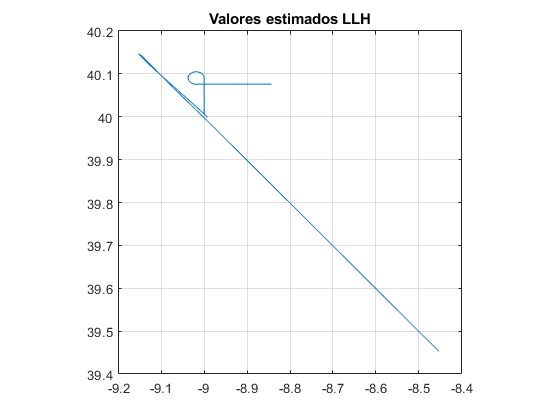
\includegraphics[width=0.8\textwidth]{kalman_3/2-3-plot_posicao_estimada_LLH.png}
	\caption{Kalman,Posição Estimada com Ionosfera e sem Canyon.}
	\label{Posicao23}
\end{figure}

\begin{figure}[ht]
	\centering
	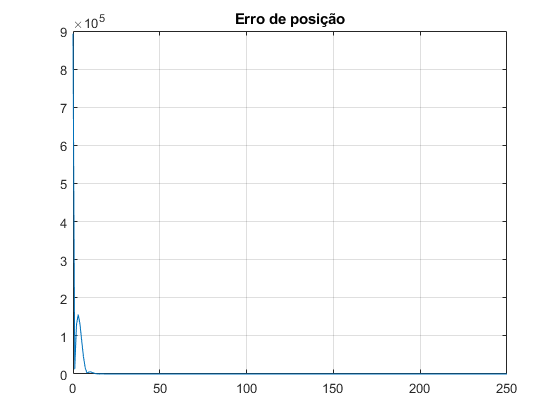
\includegraphics[width=0.8\textwidth]{kalman_3/2-3-erro_posicao.png}
	\caption{Kalman, Erro de Posição Estimada com Ionosfera e sem Canyon.}
	\label{ePosicao23}
\end{figure}

\begin{figure}[ht]
	\centering
	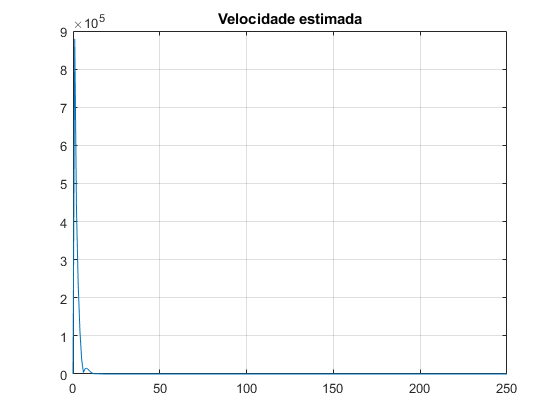
\includegraphics[width=0.8\textwidth]{kalman_3/2-3-velocidade_estimada.png}
	\caption{Kalman, Velocidade Estimada com Ionosfera e sem Canyon.}
	\label{Velocidade23}
\end{figure}


\begin{figure}[ht]
	\centering
	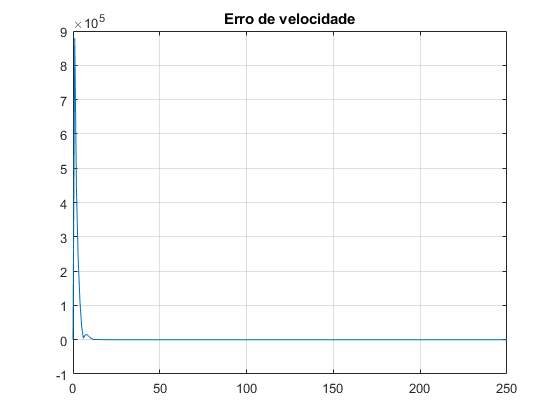
\includegraphics[width=0.8\textwidth]{kalman_3/2-3-erro_velocidade.png}
	\caption{Kalman, Erro de Velocidade Estimada com Ionosfera e sem Canyon.}
	\label{eVelocidade23}
\end{figure}

\begin{figure}[ht]
	\centering
	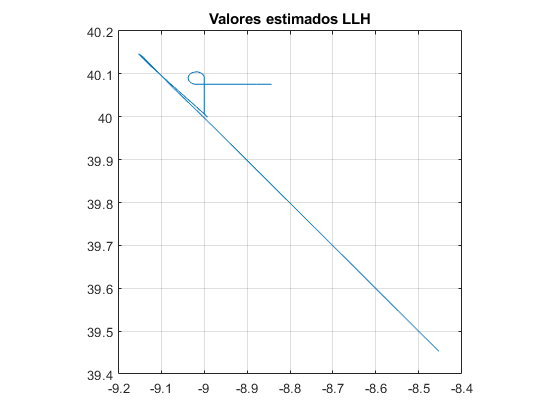
\includegraphics[width=0.8\textwidth]{kalman_4/2-4-plot_posicao_estimada_LLH.png}
	\caption{Kalman,Posição Estimada sem Ionosfera e sem Canyon.}
	\label{Posicao24}
\end{figure}

\begin{figure}[ht]
	\centering
	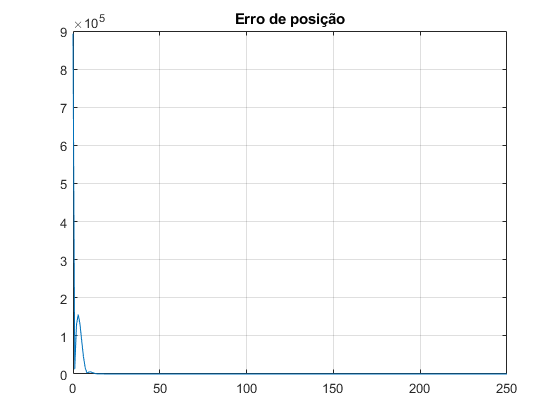
\includegraphics[width=0.8\textwidth]{kalman_4/2-4-erro_posicao.png}
	\caption{Kalman, Erro Posição Estimada sem Ionosfera e sem Canyon.}
	\label{ePosicao24}
\end{figure}

\begin{figure}[ht]
	\centering
	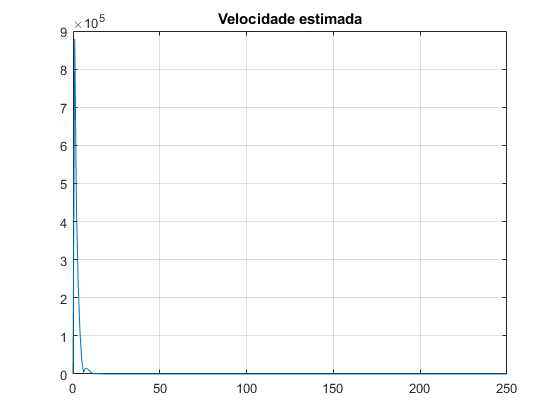
\includegraphics[width=0.8\textwidth]{kalman_4/2-4-velocidade_estimada.png}
	\caption{Kalman, Velocidade Estimada sem Ionosfera e sem Canyon.}
	\label{velocidade24}
\end{figure}


\begin{figure}[ht]
	\centering
	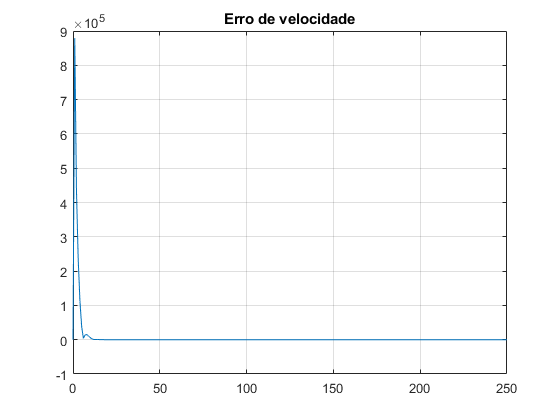
\includegraphics[width=0.8\textwidth]{kalman_4/2-4-erro_velocidade.png}
	\caption{Kalman, Erro de Velocidade Estimada sem Ionosfera e sem Canyon.}
	\label{evelocidade24}
\end{figure}

\FloatBarrier

Finda a análise anterior, procedeu-se ao cálculo dos valores RMS dos erros de posição e velocidade. Os resultados obtidos estão presentes nas tabelas seguintes. Todos os valores foram obtidos usando 5 satélites para minimização do PDOP e variância do ruído de $3.162278$.

\begin{table}[ht]
    \centering
    
    \begin{tabular}{c c c}\toprule
        \textbf{Análise} & \textbf{Erro RMS} &\textbf{Erro RMS desprezando a primeira estimação}\\
        \midrule
        Com Ionosfera e com Canyon & $37.009329$ & $37.011663$\\
        Sem Ionosfera e com Canyon & $13.656877$ & $13.683035$\\
        Com Ionosfera e sem Canyon & $37.149378$ & $37.150565$\\
        Sem Ionosfera e sem Canyon & $2.534119$ & $2.509557$ \\
        \bottomrule
    \end{tabular}
    \caption{Erro RMS de posição para as diversas condições usando o método dos mínimos quadrados}
    \label{tab:something}
    
\end{table}

\begin{table}[ht]
    \centering
    \begin{tabular}{c c c}\toprule
        \textbf{Análise} & \textbf{Erro RMS} &\textbf{Erro RMS desprezando a primeira estimação}\\
        \midrule
        Com Ionosfera e com Canyon & $6457.602631$ & $9.006785$\\
        Sem Ionosfera e com Canyon & $6457.208998$ & $8.527335$\\
        Com Ionosfera e sem Canyon & $6457.393631$ & $1.396776$\\
        Sem Ionosfera e sem Canyon & $6457.274203$ & $1.505875$ \\
        \bottomrule
    \end{tabular}
    \caption{Erro RMS de velocidade para as diversas condições usando o método dos mínimos quadrados}
    \label{tab:something}
\end{table}


\begin{table}[ht]
    \centering
    \begin{tabular}{c c c}\toprule
        \textbf{Análise} & \textbf{Erro RMS} &\textbf{Erro RMS desprezando as primeiras estimações}\\
        \midrule
        Com Ionosfera e com Canyon & $58859.804735$ & $40.668595$\\
        Sem Ionosfera e com Canyon & $58858.647870$ & $8.457399$\\
        Com Ionosfera e sem Canyon & $58859.918390$ & $34.971260$\\
        Sem Ionosfera e sem Canyon & $58858.602337$ & $8.403958$ \\
        \bottomrule
    \end{tabular}
    \caption{Erro RMS de posição para as diversas condições usando filtro de Kalman}
    \label{tab:something}
\end{table}

\begin{table}[ht]
    \centering
    \begin{tabular}{c c c}\toprule
        \textbf{Análise} & \textbf{Erro RMS} &\textbf{Erro RMS desprezando as primeiras estimações}\\
        \midrule
        Com Ionosfera e com Canyon & $64215.927545$ & $3.609797$\\
        Sem Ionosfera e com Canyon & $64215.682332$ & $1.671280$\\
        Com Ionosfera e sem Canyon & $64216.108580$ & $3.415421$\\
        Sem Ionosfera e sem Canyon & $64215.855161$ & $1.634545$ \\
        \bottomrule
    \end{tabular}
    \caption{Erro RMS de velocidade para as diversas condições usando filtro de Kalman}
    \label{tab:something}
\end{table}

Para comparar ambos os algoritmos melhor, podemos realizar 100 iterações e obter o erro RMS médio das mesmas. Nas condições iniciais do projecto, obtiveram-se os seguintes resultados presentes nas Tabelas \ref{tab:something1} e \ref{tab:something2}.
\begin{table}[ht]
    \centering
    %\begin{adjustbox}{max width=\textwidth}
    \begin{tabular}{c c c}\toprule
        \textbf{Método} & \textbf{Erro RMS médio} &\textbf{Erro RMS médio desprezando as primeiras estimações}\\
        \midrule
        Mínimos Quadrados & $2.454870$ & $2.455320$\\
        Extended Kalman Filter & $58859.924500$ & $42.434591$\\
        \bottomrule
    \end{tabular}
    %\end{adjustbox}
    \caption{Erro RMS de posição para os dois métodos}
    \label{tab:something1}
\end{table}

\begin{table}[ht]
    \centering
    %\begin{adjustbox}{max width=\textwidth}
    \begin{tabular}{c c c}\toprule
        \textbf{Método} & \textbf{Erro RMS médio} &\textbf{Erro RMS médio desprezando as primeiras estimações}\\
        \midrule
        Mínimos Quadrados & $6457.173675$ & $1.491769$\\
        Extended Kalman Filter & $64216.093992$ & $3.732317$\\
        \bottomrule
    \end{tabular}
    %\end{adjustbox}
    \caption{Erro RMS de velocidade para os dois métodos}
    \label{tab:something2}
\end{table}

Para comparar ambos os algoritmos melhor, podemos realizar 100 iterações e obter o erro RMS médio das mesmas. Nas condições iniciais do projecto, obtiveram-se os seguintes resultados presentes nas Tabelas \ref{tab:something1} e \ref{tab:something2}.
\begin{table}[ht]
    \centering
    %\begin{adjustbox}{max width=\textwidth}
    \begin{tabular}{c c c}\toprule
        \textbf{Método} & \textbf{Erro RMS médio} &\textbf{Erro RMS médio desprezando as primeiras estimações}\\
        \midrule
        Mínimos Quadrados & $2.454870$ & $2.455320$\\
        Extended Kalman Filter & $58859.924500$ & $42.434591$\\
        \bottomrule
    \end{tabular}
    %\end{adjustbox}
    \caption{Erro RMS de posição para os dois métodos}
    \label{tab:something1}
\end{table}

\begin{table}[ht]
    \centering
    %\begin{adjustbox}{max width=\textwidth}
    \begin{tabular}{c c c}\toprule
        \textbf{Método} & \textbf{Erro RMS médio} &\textbf{Erro RMS médio desprezando as primeiras estimações}\\
        \midrule
        Mínimos Quadrados & $6457.173675$ & $1.491769$\\
        Extended Kalman Filter & $64216.093992$ & $3.732317$\\
        \bottomrule
    \end{tabular}
    %\end{adjustbox}
    \caption{Erro RMS de velocidade para os dois métodos}
    \label{tab:something2}
\end{table}

Podemos também obter a comparação dos métodos em cada segmento da trajectória, como se pode ver nas Tabelas \ref{tab:something3} e \ref{tab:something4}. Note-se que no segmento AB se desprezaram as primeiras estimações para ambos os métodos.

\begin{table}[ht]
    \centering
    %\begin{adjustbox}{max width=\textwidth}
    \begin{tabular}{c c c}\toprule
        \textbf{Segmento} & \textbf{Erro RMS médio MMQ} &\textbf{Erro RMS médio Kalman}\\
        \midrule
        AB & $37.950455$ & $37.173439$\\
        BC & $41.393124$ & $37.164251$ \\
        CD & $32.126496$ & $37.138547$ \\
        DE & $56.947079$ & $36.577543$\\
        \bottomrule
    \end{tabular}
    %\end{adjustbox}
    \caption{Erro RMS de posição para os dois métodos, separado por segmentos}
    \label{tab:something3}
\end{table}

\begin{table}[h]
    \centering
    %\begin{adjustbox}{max width=\textwidth}
    \begin{tabular}{c c c}\toprule
        \textbf{Segmento} & \textbf{Erro RMS médio MMQ} &\textbf{Erro RMS médio Kalman}\\
        \midrule
        AB & $4.207579$ & $1.627670$\\
        BC & $4.495119$ & $1.520109 $ \\
        CD & $2.167333$ & $1.315903 $ \\
        DE & $3.225688$ & $18.657377 $ \\
        \bottomrule
    \end{tabular}
    %\end{adjustbox}
    \caption{Erro RMS de velocidade para os dois métodos, separado por segmentos}
    \label{tab:something4}
\end{table}

\FloatBarrier


\section{Conclusões}

Para todas as simulações foi usada a mesma constelação, sendo que nas condições da simulação tivemos sempre em vista (ou seja, com elevação superior a 10º) 12 satélites, como podemos ver na Figura \ref{satelites1}.

Nestas simulações verificamos que os erros apresentam uma grande dependência dos satélites usados para determinar a posição. Ao forçar o uso de sub-constelações de 5 satélites que minimizam o parâmetro PDOP verificamos que ambos os algoritmos implementados apresentam boas estimativas de posição, no entanto essa estimativa torna-se muito menos aceitável quando se força o uso de apenas 4 satélites com as elevações mais altas, forçando o simulador a usar um parâmetro PDOP muito pior.  

Para os outros parâmetros, $\rho_{iono}$ e $n_{m}(t)$, esta dependência é muito inferior. Assim, a minimização do parâmetro PDOP é da maior importância para uma boa estimação da posição.

Para as estimações de posição, verificamos que o método dos mínimos quadrados apresenta erros ligeiramente superiores aos do filtro de Kalman, embora estejam ainda na mesma ordem de grandeza. Esta melhoria da precisão deve-se principalmente ao método de Kalman implementado ter como estado a velocidade da aeronave, permitindo-lhe uma maior precisão na estimação da posição. Há que no entanto ter em conta que o método dos mínimos quadrados apresenta um erro menor nas primeiras iterações em comparação ao filtro de Kalman, que demora mais tempo a ter uma estimação aceitável.

Para as estimações de velocidade, verificamos que o método dos mínimos quadrados apresenta erros elevados. O filtro de Kalman apresenta erros de velocidade melhores, mas também algo elevados. Nas condições do problema, estes métodos são de baixa utilidade prática em situações que a determinação da velocidade em tempo real seja relevante, embora possam ser adequados para usos que requeiram menos precisão.

\pagebreak
\section{Referências}
\nocite{*}
 \printbibliography

\pagebreak
\appendix
\section{Anexos}
\subsection{Mínimos quadrados}
\subsection{\texttt{circular\_motion.m}}
\inputminted[fontsize=\footnotesize]{matlab}{code_LS/circular_motion.m}

\subsection{\texttt{compute\_LS\_solution.m}}
\inputminted[fontsize=\footnotesize]{matlab}{code_LS/compute_LS_solution.m}

\subsection{\texttt{compute\_orbital\_parameters.m}}
\inputminted[fontsize=\footnotesize]{matlab}{code_LS/compute_orbital_parameters.m}

\subsection{\texttt{compute\_pseudoranges.m}}
\inputminted[fontsize=\footnotesize]{matlab}{code_LS/compute_pseudoranges.m}

\subsection{\texttt{compute\_satellite\_position.m}}
\inputminted[fontsize=\footnotesize]{matlab}{code_LS/compute_satellite_position.m}

\subsection{\texttt{compute\_true\_range.m}}
\inputminted[fontsize=\footnotesize]{matlab}{code_LS/compute_true_range.m}

\subsection{\texttt{ECEF2ENU.m}}
\inputminted[fontsize=\footnotesize]{matlab}{code_LS/ECEF2ENU.m}

\subsection{\texttt{ENU2AzEl.m}}
\inputminted[fontsize=\footnotesize]{matlab}{code_LS/ENU2AzEl.m}

\subsection{\texttt{ENU2ECEF.m}}
\inputminted[fontsize=\footnotesize]{matlab}{code_LS/ENU2ECEF.m}

\subsection{\texttt{filter\_satellites\_visible\_LS.m}}
\inputminted[fontsize=\footnotesize]{matlab}{code_LS/filter_satellites_visible_LS.m}

\subsection{\texttt{flat2llh.m}}
\inputminted[fontsize=\footnotesize]{matlab}{code_LS/flat2llh.m}

\subsection{\texttt{linear\_motion.m}}
\inputminted[fontsize=\footnotesize]{matlab}{code_LS/linear_motion.m}

\subsection{\texttt{LLH2XYZ.m}}
\inputminted[fontsize=\footnotesize]{matlab}{code_LS/LLH2XYZ.m}

\subsection{\texttt{main\_least\_squares.m}}
\inputminted[fontsize=\footnotesize]{matlab}{code_LS/main_least_squares.m}

\subsection{\texttt{minimize\_PDOP.m}}
\inputminted[fontsize=\footnotesize]{matlab}{code_LS/minimize_PDOP.m}

\subsection{\texttt{read\_yuma.m}}
\inputminted[fontsize=\footnotesize]{matlab}{code_LS/read_yuma.m}

\subsection{\texttt{update\_position.m}}
\inputminted[fontsize=\footnotesize]{matlab}{code_LS/update_position.m}

\subsection{\texttt{XYZ2LLH.m}}
\inputminted[fontsize=\footnotesize]{matlab}{code_LS/XYZ2LLH.m}

%%%%%%%%%%%%%%%%%%%%%%%%%%%%%%%%%%%%%%%
\subsection{Filtro de Kalmam}
\subsection{\texttt{circular\_motion.m}}
\inputminted[fontsize=\footnotesize]{matlab}{code_kalman/circular_motion.m}

\subsection{\texttt{compute\_orbital\_parameters.m}}
\inputminted[fontsize=\footnotesize]{matlab}{code_kalman/compute_orbital_parameters.m}

\subsection{\texttt{compute\_pseudoranges.m}}
\inputminted[fontsize=\footnotesize]{matlab}{code_kalman/compute_pseudoranges.m}

\subsection{\texttt{compute\_satellite\_position.m}}
\inputminted[fontsize=\footnotesize]{matlab}{code_kalman/compute_satellite_position.m}

\subsection{\texttt{compute\_true\_range.m}}
\inputminted[fontsize=\footnotesize]{matlab}{code_kalman/compute_true_range.m}

\subsection{\texttt{ECEF2ENU.m}}
\inputminted[fontsize=\footnotesize]{matlab}{code_kalman/ECEF2ENU.m}

\subsection{\texttt{ENU2AzEl.m}}
\inputminted[fontsize=\footnotesize]{matlab}{code_kalman/ENU2AzEl.m}

\subsection{\texttt{ENU2ECEF.m}}
\inputminted[fontsize=\footnotesize]{matlab}{code_kalman/ENU2ECEF.m}

\subsection{\texttt{filter\_satellites\_visible\_KALMAN.m}}
\inputminted[fontsize=\footnotesize]{matlab}{code_kalman/filter_satellites_visible_KALMAN.m}

\subsection{\texttt{flat2llh.m}}
\inputminted[fontsize=\footnotesize]{matlab}{code_kalman/flat2llh.m}

\subsection{\texttt{kalman\_main.m}}
\inputminted[fontsize=\footnotesize]{matlab}{code_kalman/kalman_main.m}

\subsection{\texttt{linear\_motion.m}}
\inputminted[fontsize=\footnotesize]{matlab}{code_kalman/linear_motion.m}

\subsection{\texttt{LLH2XYZ.m}}
\inputminted[fontsize=\footnotesize]{matlab}{code_kalman/LLH2XYZ.m}

\subsection{\texttt{minimize\_PDOP.m}}
\inputminted[fontsize=\footnotesize]{matlab}{code_kalman/minimize_PDOP.m}

\subsection{\texttt{read\_yuma.m}}
\inputminted[fontsize=\footnotesize]{matlab}{code_kalman/read_yuma.m}

\subsection{\texttt{update\_position.m}}
\inputminted[fontsize=\footnotesize]{matlab}{code_kalman/update_position.m}

\subsection{\texttt{XYZ2LLH.m}}
\inputminted[fontsize=\footnotesize]{matlab}{code_kalman/XYZ2LLH.m}
\end{document}
